The implementation of Catenable Lists we used can be found 
on pages 93-98 of the reference book (\cite{Okasaki}),
and the implementation for Queues, needed for their implementation, 
is described on pages 15-18.

\subsection{Data Structure Implementation Overview}
The aim of the Catenable List data structure is 
to have a List implementation with efficient concatenation, 
hence its name.
As said above, Catenable Lists are based on Queues
and for this reason we had to implement them as well.

\subsubsection{Queues Overview}
The implementation represents a Queue as two lists (left and right), 
and the order of elements in the Queue is the order of the left list, 
followed by the reverse order of the right list.
The operations implementations are easy to deduce from that: 
we add elements on the right list (with \verb|snoc|) 
and remove them from the left list (with \verb|head|).
At some point, the right list must obviously be reversed and put on the left.
In our case, in order to have the \verb|head|
operation in constant time,
as is wanted in the implementation,
the invariant must be enforced that a non-empty list has a non-empty left list.
It comes from that, 
that the \verb|tail| operation must reverse the right list when the left one becomes empty, 
and \verb|snoc| must add an element on the left list of an empty Queue.

All operations are in constant time, or amortized constant time for \verb|tail|.
Let us now see an overview of the Catenable List structure.

\subsubsection{Catenable Lists Overview}
We can represent a Catenable List as a tree 
in which the order of elements can be recovered by traversing the tree in preorder.
It is implemented as an element (the root of the tree), 
and a Queue of Catenable Lists (its children).
\\
\centerline{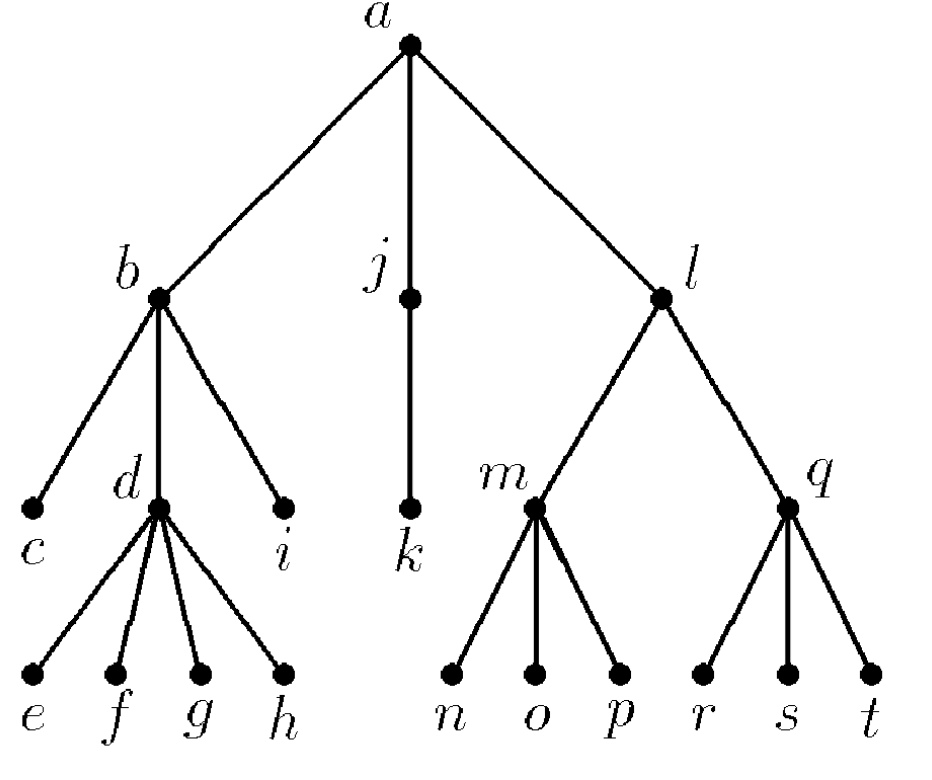
\includegraphics[scale=0.17]{preorder}}
\centerline{\emph{Illustration 1: representation of a list from a to t}}
\centerline{}
\\
The concatenation is then simply done by adding the List we want to concatenate 
at the end of the Queue of the current List 
(operation called \verb|link|).
When it comes to the other operations,
\verb|head| is trivial (it simply returns the root)
and operations adding an element at the end or beginning of the List, 
\verb|snoc| and \verb|cons|,
simply use the \verb|concatenation| operation.
The \verb|tail| operation requires 
to create a Catenable List from a Queue of Catenable Lists.
For that, it just links all Lists of the Queue 
by putting the successor of a List $l$ in the Queue at the end of $l$'s Queue.

All operations are done in amortized constant time.
Let us now see its verification with Leon.

\subsection{Verification with Leon}
In order to verify the correctness of the implementation of both data structures in Leon,
we used some functions like \verb|size|, \verb|content| and \verb|toList|.
The Queue implementation had also an invariant to be checked (explained above),
so the Catenable List implementation had to ensure that the Queues it uses 
%and creates ? %TODO 
satisfies the invariant as well.

We also wrote some tests to be evaluated that helped us to find some errors,
where we could not be precise enough in the specification of functions,
or where Leon gave \verb|Unknown|s.

The Queue implementation could be verified by Leon,
but the Catenable List implementation had some \verb|Unknown|s,
probably due to its recursive structure. Overall, we were able to verify 67 checks over 78.

In the process of verification we learned some limitations of Leon,
such as that the use of high-order functions makes verification hard if not impossible.
We had also some difficulties with mutually recursive checks, 
which made stack-overflows.

In the process, we also managed to compile Leon code directly using \verb|scalac|, 
which allowed us to test our implementation both using the \verb|--eval| option of
Leon and as a standalone program.

%TODO
%: more ?